% Created 2020-07-01 mié 08:13
% Intended LaTeX compiler: pdflatex
\documentclass[presentation,aspectratio=1610]{beamer}
\usepackage[utf8]{inputenc}
\usepackage[T1]{fontenc}
\usepackage{graphicx}
\usepackage{grffile}
\usepackage{longtable}
\usepackage{wrapfig}
\usepackage{rotating}
\usepackage[normalem]{ulem}
\usepackage{amsmath}
\usepackage{textcomp}
\usepackage{amssymb}
\usepackage{capt-of}
\usepackage{hyperref}
\usepackage{khpreamble}
\usepackage{amssymb}
\DeclareMathOperator{\shift}{q}
\DeclareMathOperator{\diff}{p}
\usetheme{default}
\author{Kjartan Halvorsen}
\date{2020-06-30}
\title{Computerized Control - difference equations, LSI, impulse response}
\hypersetup{
 pdfauthor={Kjartan Halvorsen},
 pdftitle={Computerized Control - difference equations, LSI, impulse response},
 pdfkeywords={},
 pdfsubject={},
 pdfcreator={Emacs 26.3 (Org mode 9.3.6)}, 
 pdflang={English}}
\begin{document}

\maketitle

\section{Intro: Discrete-time signals and systems}
\label{sec:orgfd81190}
\begin{frame}[label={sec:orgef7f664}]{Position control of a diskdrive arm}
\begin{columns}
\begin{column}{0.5\columnwidth}
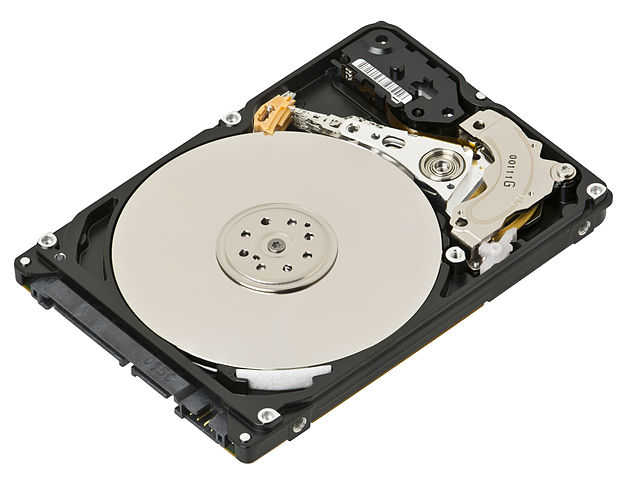
\includegraphics[height=0.5\textheight]{../../figures/diskdrive.png}

\tiny "Laptop-hard-drive-exposed" by Evan-Amos - Own work. Licensed under CC BY-SA 3.0 via Commons
\end{column}
\begin{column}{0.5\columnwidth}
\[ J\ddot{\theta}(t) = u(t) + v(t) \]
\begin{center}
  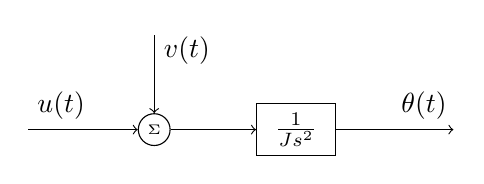
\begin{tikzpicture}[node distance=22mm, block/.style={rectangle, draw, minimum width=10mm}, sumnode/.style={circle, draw, inner sep=2pt}]

    \node[coordinate] (input) {};
    \node[sumnode, right of=input, node distance=16mm] (sum) {\tiny $\Sigma$};
    \node[block, right of=sum, node distance=18mm] (plant)  {$\frac{1}{Js^2}$};
    \node[coordinate, above of=sum, node distance=12mm] (disturbance) {};
    \node[coordinate, right of=plant, node distance=20mm] (output) {};

    \draw[->] (input) -- node[above, pos=0.3] {$u(t)$} (sum);
    \draw[->] (sum) -- node[above] {} (plant);
    \draw[->] (plant) -- node[above, near end] {$\theta(t)$} (output);
    \draw[->] (disturbance) -- node[right, pos=0.2] {$v(t)$} (sum);
  \end{tikzpicture}
\end{center}
\end{column}
\end{columns}
\end{frame}

\begin{frame}[label={sec:orgdfbfff8}]{Two approaches to designing a  discrete-time controller}
\begin{enumerate}
\item Do design the controller in the continuous-time domain (methods from control engineering class). Then discretize the continuous-time controller.
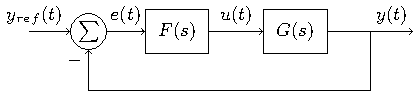
\includegraphics[width=0.7\linewidth]{../../figures/block1} \(F_d(z) \approx F(s)\)
\item Determine discrete-time model of the plant. Do design in discrete-time domain.
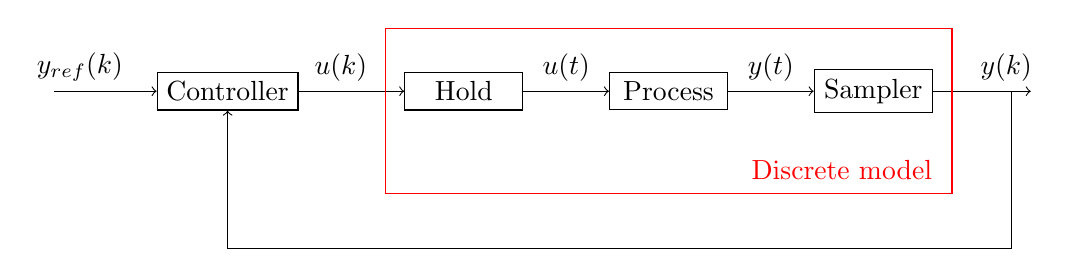
\begin{tikzpicture}[node distance=22mm, block/.style={rectangle, draw, minimum width=15mm}, sumnode/.style={circle, draw, inner sep=2pt}]

  \node[coordinate,] (refinput) {};
  \node[block, right of=refinput] (controller)  {Controller};
  \node[block, right of=controller, node distance=30mm] (zoh)  {Hold};
  \node[block, right of=zoh, node distance=26mm] (plant)  {Process};
  \node[block, right of=plant, node distance=26mm] (sampler)  {Sampler};
  \node[coordinate, right of=sampler, node distance=20mm] (output) {};

  \draw[->] (refinput) -- node[above, near start] {$y_{ref}(k)$} (controller);
  \draw[->] (controller) -- node[above, pos=0.4] {$u(k)$} (zoh);
  \draw[->] (zoh) -- node[above] {$u(t)$} (plant);
  \draw[->] (plant) -- node[above] {$y(t)$} (sampler);
  \draw[->] (sampler) -- node[pos=0.8, coordinate] (measure) {} node[above, near end] {$y(k)$} (output);
  \draw[->] (measure) -- ++(0,-20mm) -| (controller);
  \draw[red] (42mm, -13mm) rectangle (114mm, 8mm);
  \node[red] at (100mm, -10mm) {Discrete model};
\end{tikzpicture}
\end{enumerate}
\end{frame}


\begin{frame}[label={sec:org2b78030}]{Difference equations}
We saw two difference equations in the introductory lecture

\begin{enumerate}
\item Discretized version of continuous-time lead-compensator \(F(s)=K\frac{s+b}{s+a}\)
\begin{center}
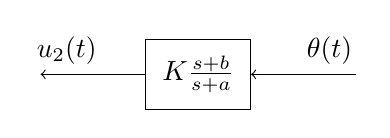
\begin{tikzpicture}
\node[draw, inner sep=6pt] (block) {$K\frac{s+b}{s+a}$};
\draw[->] (block) ++ (2,0) -- node[above, near start] {$\theta(t)$} (block);
\draw[->] (block) -- node[above, near end] {$u_2(t)$}  ++(-2,0);
\end{tikzpicture}
\end{center}
\[ u_2(kh+h) - (1-ah)u_2(kh) = K\theta(kh+h) - K(1-bh)\theta(kh) \]
\item Discretized version of the double integrator \(G(s)=\frac{1}{Js^2}\)
\begin{center}
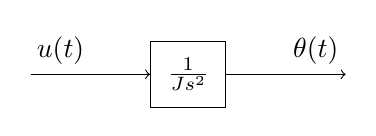
\begin{tikzpicture}
\node[draw, inner sep=6pt] (block) {$\frac{1}{Js^2}$};
\draw[<-] (block) ++ (2,0) -- node[above, near start] {$\theta(t)$} (block);
\draw[<-] (block) -- node[above, near end] {$u(t)$}  ++(-2,0);
\end{tikzpicture}
\end{center}
\[ \theta(k+2) - 2\theta(k+1) + \theta(k) = \frac{h^2}{J} u(k)\]
\end{enumerate}
\end{frame}

\begin{frame}[label={sec:orgfde4f26}]{Direct solution by iteration}
The difference equation can be used as a recipe to calculate the solution numerically

\alert{Example} Calculate the response of the lead-compensator \(u_2(kh+h) - (1-ah)u_2(kh) = K\theta(kh+h) - K(1-bh)\theta(kh)\) with \(a=8\), \(b=1\), \(h=0.1\), \(K=1\)
to the signal below
\begin{center}
  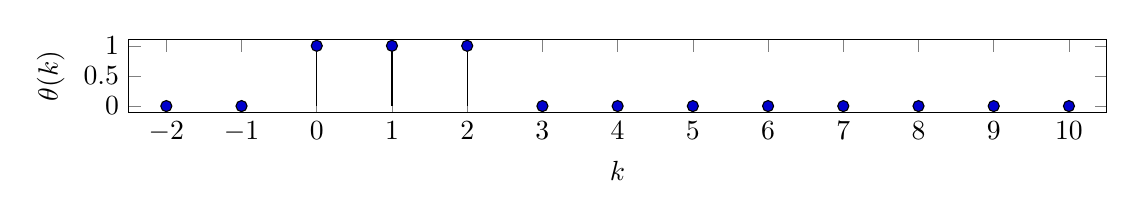
\begin{tikzpicture}
    \begin{axis}[
      width=14cm,
      height=2.5cm,
      xlabel={$k$},
      ylabel={$\theta(k)$},
      xmin=-2.5,
      xmax=10.5,
      ]

      \addplot+[black, ycomb, domain=-2:10, samples=13,variable=k] { (k>=0)*(k<3) }; 

    \end{axis}
  \end{tikzpicture}
\end{center}
\begin{align*}
     u_2(k+1) &= 0.2u_2(k) + \theta(k+1) - 0.9\theta(k)\\
     u_2(0) &= 0.2u_2(-1) + \theta(0) - 0.9\theta(-1) = 0 + 1 -0 = 1\\
     u_2(1) &= 0.2u_2(0) + \theta(1) - 0.9\theta(0) = 0.2 + 1 - 0.9 = 0.3\\
     u_2(2) &= 0.2u_2(1) + \theta(2) - 0.9\theta(1) = 0.06 + 1 - 0.9 = 0.16\\
     u_2(3) &= 0.2u_2(2) + \theta(3) - 0.9\theta(2) = 0.032 + 0 - 0.9 = -0.868\\
     u_2(4) &= 0.2u_2(3) + \theta(4) - 0.9\theta(3) = -0.1736 + 0 - 0 = -0.1736\\
\end{align*}
\end{frame}

\begin{frame}[label={sec:org106b5e1}]{Direct solution by iteration}
\begin{block}{Input}
\begin{center}
  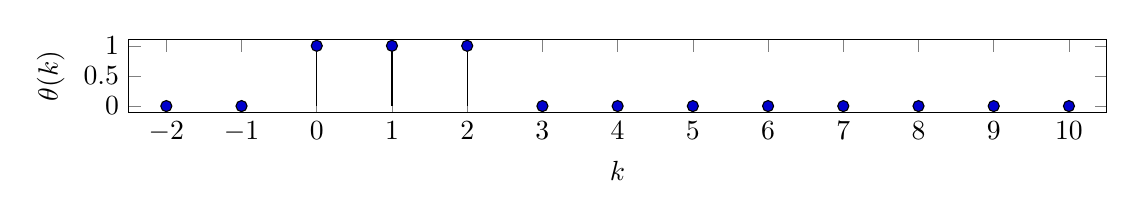
\begin{tikzpicture}
    \begin{axis}[
      width=14cm,
      height=2.5cm,
      xlabel={$k$},
      ylabel={$\theta(k)$},
      xmin=-2.5,
      xmax=10.5,
      ]

      \addplot+[black, ycomb, domain=-2:10, samples=13,variable=k] { (k>=0)*(k<3) }; 

    \end{axis}
  \end{tikzpicture}
\end{center}
\end{block}

\begin{block}{Output}
\begin{center}
  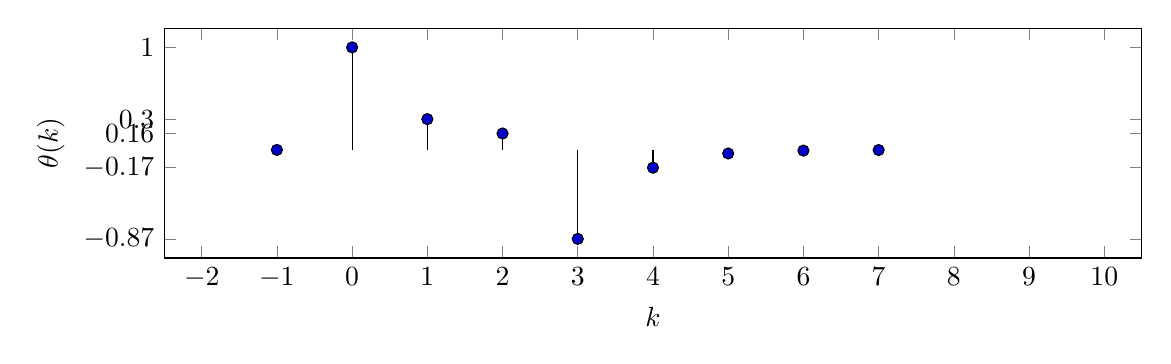
\begin{tikzpicture}
    \begin{axis}[
      width=14cm,
      height=4.5cm,
      xlabel={$k$},
      ylabel={$\theta(k)$},
      ytick={-0.868, -0.1736, 0.16, 0.3, 1},
      xmin=-2.5,
      xmax=10.5,
      ]
      \addplot+[black, ycomb] coordinates {(-1,0) (0,1) (1, 0.3) (2,0.16) (3,-0.868)
	                                   (4,-0.1736) (5,-0.035) (6,-0.007) (7,-0.0014)}; 
    \end{axis}
  \end{tikzpicture}
\end{center}
\end{block}
\end{frame}
\begin{frame}[label={sec:org6571ae1}]{Do on your own: Solution to the discrete double-integrator}
\alert{Activity} Calculate the response of the double-integrator 
\[ \theta(k+2) - 2\theta(k+1) + \theta(k) = \frac{h^2}{J} u(k)\]
with \(h=1\), \(J=1\) 

and initial values zero: \(\theta(k) = 0, \; k \le 0\) 
to the signal below
\begin{center}
  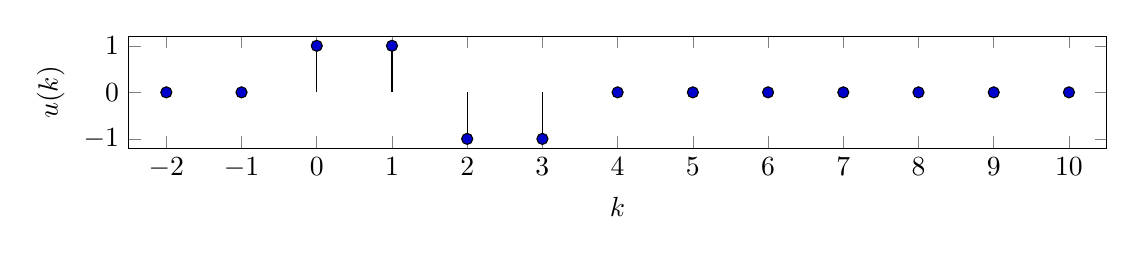
\begin{tikzpicture}
    \begin{axis}[
      width=14cm,
      height=3cm,
      xlabel={$k$},
      ylabel={$u(k)$},
      xmin=-2.5,
      xmax=10.5,
      ]

      \addplot+[black, ycomb, domain=-2:10, samples=13,variable=k] { (k>=0)*(k<2) - (k>=2)*(k<4) }; 
    \end{axis}
  \end{tikzpicture}
\end{center}

Sketch your solution as a graph on paper, photograph and send as PM on Remind.
\end{frame}

\begin{frame}[label={sec:orgfcb06cf}]{Do on your own: Solution to the discrete double-integrator}
\alert{Solution}
\footnotesize
\[ \theta(k+2) =  2\theta(k+1) - \theta(k) + u(k)\]
and initial values zero: \( \theta(k) = 0, \; k \le 0 \) 
\begin{align*}
 \theta(0) &=  2\theta(-1) - \theta(-2) + u(-2) = 0\\
 \theta(1) &=  2\theta(0) - \theta(-1) + u(-1) = 0\\
 \theta(2) &=  2\theta(1) - \theta(0) + u(0) = 0 - 0 + 1 = 1\\
 \theta(3) &=  2\theta(2) - \theta(1) + u(1) = 2 - 0 + 1 = 3\\
 \theta(4) &=  2\theta(3) - \theta(2) + u(2) = 6 - 1 - 1 = 4\\
 \theta(5) &=  2\theta(4) - \theta(3) + u(3) = 8 - 3 - 1 = 4\\
 \theta(6) &=  2\theta(5) - \theta(4) + u(4) = 8 - 4 +0= 4\\
 \theta(7) &=  2\theta(6) - \theta(5) + u(5) = 8 - 4 +0= 4
 \end{align*}
   \begin{center}
     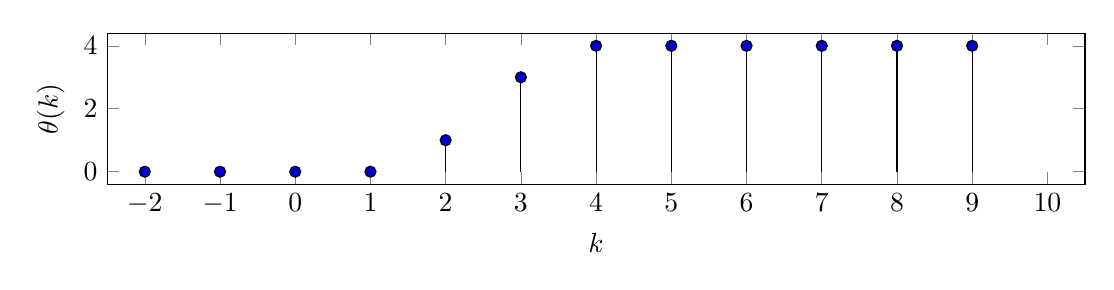
\begin{tikzpicture}
       \begin{axis}[
	 width=14cm,
	 height=3.5cm,
	 xlabel={$k$},
	 ylabel={$\theta(k)$},
	 xmin=-2.5,
	 xmax=10.5,
	 ]
	 \addplot+[black, ycomb] coordinates {(-2,0) (-1,0) (0,0) (1, 0) (2,1) (3,3)
	                                      (4, 4) (5,4) (6,4) (7,4) (8,4) (9,4)}; 
       \end{axis}
     \end{tikzpicture}
   \end{center}
\end{frame}

\begin{frame}[label={sec:org278229e}]{A short intermezzo - the shift operator}
Recall the definition of the shift operator \(\shift\):
\[ \shift f(k) = f(k+1), \quad \text{for double-infinite sequence $f(k)$} \]

\alert{Activity} Show that the discretized lead-compensator
\[ u_2(k+1) = 0.2u_2(k) + \theta(k+1) - 0.9\theta(k)\]
can be written using the shift operator as 
\[ u_2(k) = \frac{\shift -0.9}{\shift - 0.2} \theta(k).\]
\end{frame}

\begin{frame}[label={sec:orgc3ab534}]{Simple discrete-time controller for the disk drive arm}
\(J=1\) and \(h=1\) for simplicity.
\begin{center}
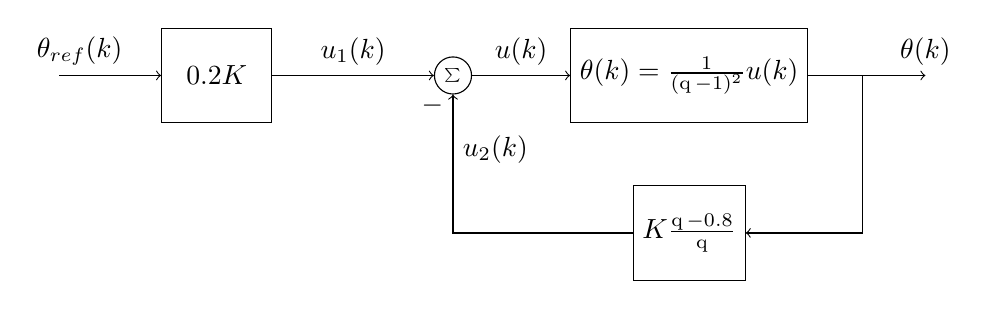
\begin{tikzpicture}
\tikzset{node distance=2cm, 
    block/.style={rectangle, draw, minimum height=12mm, minimum width=14mm},
    sumnode/.style={circle, draw, inner sep=2pt}        
}

  \node[coordinate] (input) {};
  \node[block, right of=input] (TR) {$0.2K$};
  \node[sumnode, right of=TR, node distance=30mm] (sum) {\tiny $\sum$};
  \node[block,right of=sum, node distance=30mm] (plant) {$\theta(k) = \frac{1}{(\shift-1)^2}u(k)$};
  %\node[sumnode, right of=plant, node distance=30mm] (sumdist) {$\sum$};
  %\node[coordinate, above of=sumdist, node distance=15mm] (dist) {};
  %\node[coordinate, right of=sumdist, node distance=15mm] (measure) {};
  \node[coordinate, right of=plant, node distance=30mm] (output) {};
  \node[coordinate, right of=plant, node distance=22mm] (measure) {};
  %\node[sumnode,below of=measure, node distance=25mm] (sumnoise) {$\sum$};
  %\node[coordinate, right of=sumnoise, node distance=15mm] (noise) {};
  \node[block,below of=plant, node distance=20mm] (SR) {$K\frac{\shift - 0.8}{\shift}$};

  \draw[->] (input) -- node[above, pos=0.2] {$\theta_{ref}(k)$} (TR);
  \draw[->] (TR) -- node[above] {$u_1(k)$} (sum);
  \draw[->] (sum) -- node[above] {$u(k)$} (plant);
  \draw[->] (plant) -- node[at end, above] {$\theta(k)$} (output);
  \draw[->] (measure) |- (SR);
  \draw[->] (SR) -| (sum) node[right, pos=0.8] {$u_2(k)$} node[left, pos=0.96] {$-$};
\end{tikzpicture}
\end{center}
Combine
\[ \theta(k+2) - 2\theta(k+1) + \theta(k) = u(k)\]
with the control-law
\begin{align*}
 u(k) &= u_1(k) - u_2(k)
      = 0.2K\theta_{ref}(k) - K(1 -0.8\shift^{-1})\theta(k)\\
      &=  0.2K\theta_{ref}(k) - K\big(\theta(k) -0.8\theta(k-1)\big)
\end{align*}
to get
\[ \theta(k+2) - 2\theta(k+1) + \theta(k) = 0.2K\theta_{ref}(k) - K\big(\theta(k) -0.8\theta(k-1)\big) \]
\end{frame}

\begin{frame}[label={sec:org3e8ba58}]{Simple discrete-time controller for the disk drive arm, contd}
\[ \theta(k+2) - 2\theta(k+1) + \theta(k) = 0.2K\theta_{ref}(k) - K\big(\theta(k) -0.8\theta(k-1)\big) \]
\[ \theta(k+2)-2\theta(k+1) + (1+K)\theta(k) - 0.8K\theta(k-1) = 0.2K\theta_{ref}(k)\]

The solution consists of the sum of the \alert{homogenous solution} and the \alert{particular solution}
\[ \theta(k) = \theta_H(k) + \theta_P(k) \]

\begin{block}{Homogenous solution by \alert{ansatz}: \(\theta(k) = \alpha^k\)}
\[ \theta(k+2)-2\theta(k+1) + (1+K)\theta(k) - 0.8K\theta(k-1) = 0\]
\[ \alpha^{k+2} - 2\alpha^{k+1} + (1+K)\alpha^k - 0.8K\alpha^{k-1} = 0\]
\[ (\alpha^3 - 2\alpha^2 + (1+K)\alpha - 0.8K) \alpha^{k-1} = 0\]
A non-trivial solution \(\alpha \neq 0\) requires that the paranthesis is zero:
\[ \text{\bf Characteristic equation:} \quad \alpha^3 - 2\alpha^2 + (1+K)\alpha - 0.8K = 0\]
\end{block}
\end{frame}


\begin{frame}[label={sec:orgd35bd0a}]{Simple discrete-time controller for the disk drive arm, contd}
The characteristic equation 
   \[ \alpha^3 - 2\alpha^2 + (1+K)\alpha - 0.8K = 0\]

is of \alert{third} order and will  therefore have \alert{three} solutions \(\alpha_1\),  \(\alpha_2\) and \(\alpha_3\). These are the \alert{POLES} of  the closed-loop system!

The homogenous solution will consist of the linear combination
\[ \theta_H(k) = c_1 \alpha_1^k + c_2\alpha_2^k + c_3\alpha_3^k.\]
The solution will be stable if and only if 
\[ |\alpha_j| < 1, \quad j=1,2,3\]
\end{frame}

\begin{frame}[label={sec:org95e5c27}]{Simple discrete-time controller for the disk drive arm, contd}
Studying the characteristic equation using a root locus 
\[ \alpha(\alpha -1)^2 + K(\alpha - 0.8) = 0\]
\alert{Group activity} Complete the root locus and choose a set of reasonable poles for the closed-loop system!

\begin{center}
  \begin{tikzpicture}[scale=4]
    \draw[->] (-1.2, 0) -- (1.2,0);
    \draw[->] (0, -1.2) -- (0,1.2);
    \node[red, pin=45:{2 plant poles}] at (1,0) {\large $\times$};
    \node[red, pin=135:{controller pole}] at (0,0) {\large $\times$};
    \node[green!70!black, pin=-145:{controller zero}] at (0.8,0) {\Large $\circ$};
    \node at (0.8, -0.2) {$0.8$};
    \node at (1, -0.2) {$1$};
    \draw[domain=0:360, samples=361, dashed] plot ({cos(\x)}, {sin(\x)});
    \node[coordinate, pin=60:{$|\alpha|=1$}] at (0.5, 0.87) {};
  \end{tikzpicture}
\end{center}
\end{frame}

\begin{frame}[label={sec:org5c63bde}]{Simple discrete-time controller for the disk drive arm, solution}
\begin{center}
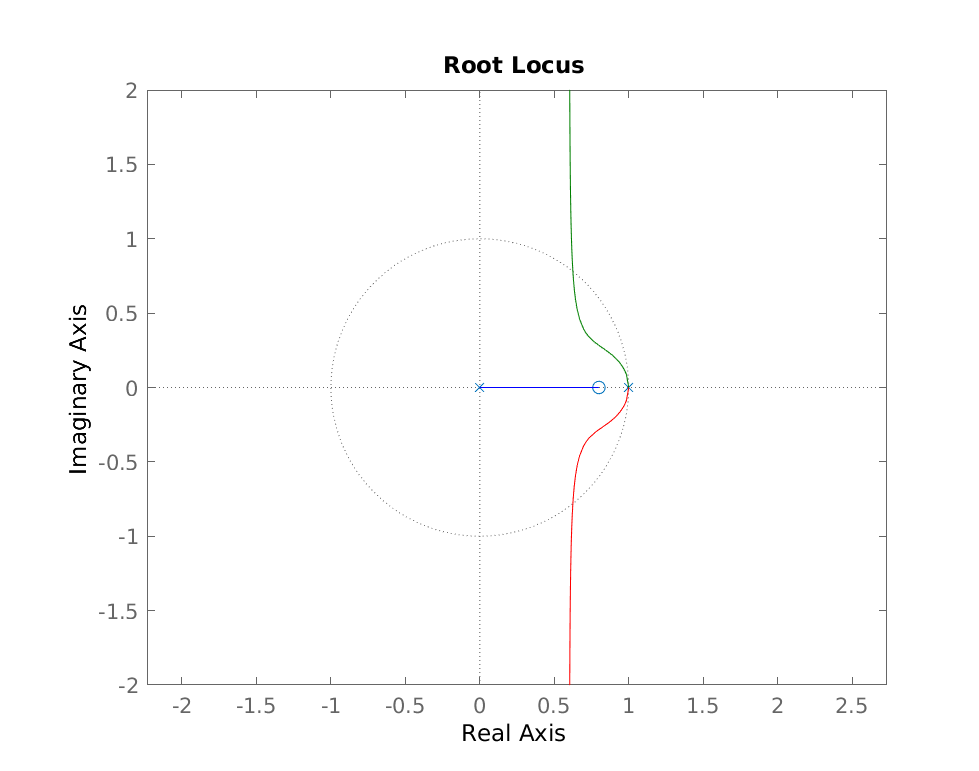
\includegraphics[width=0.8\linewidth]{rlocus-disk-arm.discrete}
\end{center}
\end{frame}


\section{Properties of discrete-time systems}
\label{sec:org825f393}

\begin{frame}[label={sec:org1aa886f}]{Sampled systems are \alert{not} time invariant}
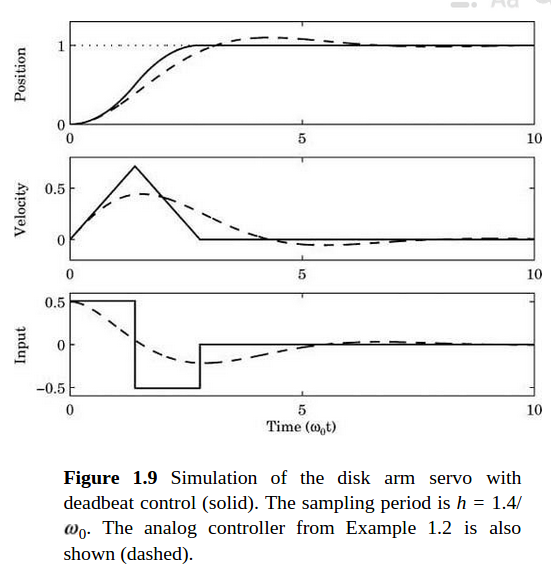
\includegraphics[height=0.6\linewidth]{../../figures/fig1-9.png}
\end{frame}

\begin{frame}[label={sec:org6c1e48c}]{The discrete-time causal linear shift-invariant system}
\begin{center}
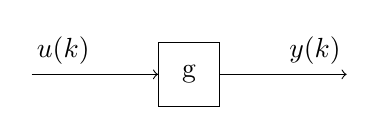
\begin{tikzpicture}[node distance=20mm, anchor=north]
\node[coordinate] (input) {};
\node[rectangle, draw, right of=input, inner sep=3mm] (lti) {g};
\node[coordinate, right of=lti] (output) {};
\draw[->] (input) -- node[near start, above] {$u(k)$}  (lti);
\draw[->] (lti) -- node[near end, above] {$y(k)$} (output);
\end{tikzpicture}
\end{center}

\(g(k)\) is called the \alert{weighting sequence}.

\begin{block}{General (non-causal) LSI}
\[ y(k) = g \ast u = \sum_{n=-\infty}^\infty g(n) u(k-n) \]
\end{block}

\begin{block}{Causal LSI}
\[ y(k) = g \ast u = \sum_{n=0}^\infty g(n) u(k-n) \]
\end{block}
\end{frame}

\begin{frame}[label={sec:org924df25}]{The discrete-time causal linear shift-invariant system}
\begin{block}{Impulse response}
If input signal is a unit pulse

\begin{center}
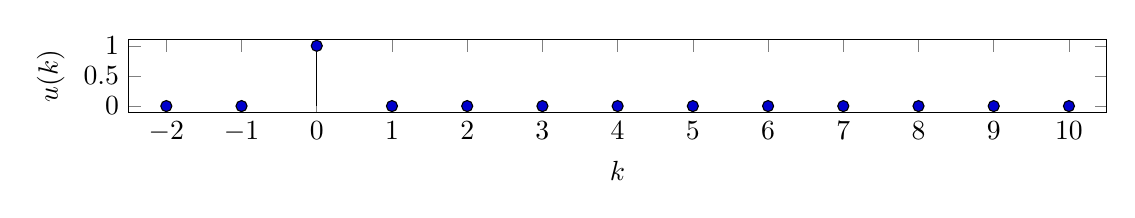
\begin{tikzpicture}
\begin{axis}[
  width=14cm,
  height=2.5cm,
  xlabel={$k$},
  ylabel={$u(k)$},
  xmin=-2.5,
  xmax=10.5,
]

\addplot+[black, ycomb, domain=-2:10, samples=13,variable=k] { (k==0)}; 

\end{axis}
\end{tikzpicture}
\end{center}

\vspace*{-5mm}


\[ y(k) = \sum_{n=0}^\infty g(n) \delta(k-n) = g(k) \]
\end{block}
\end{frame}

\begin{frame}[label={sec:orgc5e7b8c}]{The output of a causal, linear discrete-time system is a weighted sum of previous input}
\[ y(k) = g \ast u = \sum_{n=0}^\infty g(n) u(k-n) \]
The \alert{weighting sequence} \(g(k)\) is the \alert{impulse response} of the system.

What if the weighting sequence looks like this

\begin{center}
\begin{tikzpicture}
\small
\begin{axis}[
  width=14cm,
  height=3.5cm,
  xlabel={$k$},
  ylabel={$g(k)$},
  xmin=-0.5,
  xmax=10.5,
  ytick = {0, 1},
]

\addplot+[black, ycomb, domain=-2:10, samples=13,variable=k] { (k==4)}; 

\end{axis}
\end{tikzpicture}
\end{center}

\[y(k) = \]
\end{frame}

\begin{frame}[label={sec:orge36b485}]{Linearity, shift invariance and the impulse response}
The input signal

\begin{center}
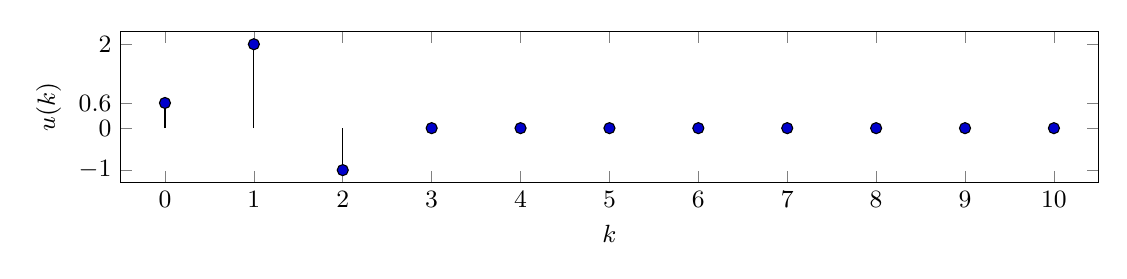
\begin{tikzpicture}
\small
\begin{axis}[
  width=14cm,
  height=3.5cm,
  xlabel={$k$},
  ylabel={$u(k)$},
  xmin=-0.5,
  xmax=10.5,
  ytick = {-1, 0, 0.6, 2},
]

\addplot+[black, ycomb, domain=-2:10, samples=13,variable=k] { 0.6*(k==0) + 2*(k==1) - 1*(k==2)}; 

\end{axis}
\end{tikzpicture}
\end{center}

Can be written 
\[u(k) = 0.6\delta(k) + 2\delta(k-1) - \delta(k-2) \]
Since the system's response to a pulse is given by \(g(k)\), the output signal is
\[ y(k) = ?\]
\end{frame}

\begin{frame}[label={sec:org1f189e0}]{Linearity, shift invariance and the impulse response}
The input signal
\begin{center}
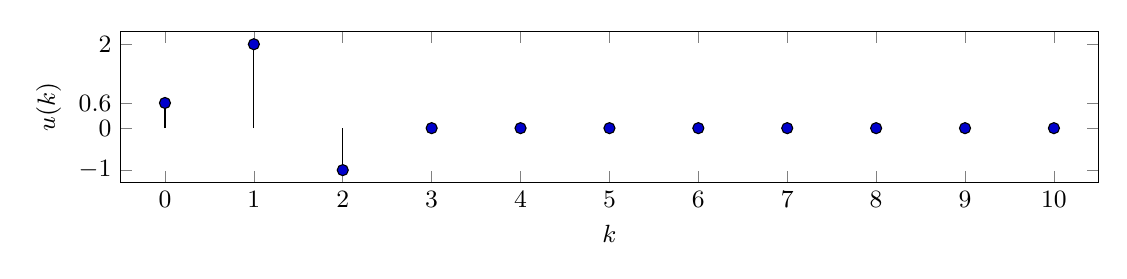
\begin{tikzpicture}
\small
\begin{axis}[
  width=14cm,
  height=3.5cm,
  xlabel={$k$},
  ylabel={$u(k)$},
  xmin=-0.5,
  xmax=10.5,
  ytick = {-1, 0, 0.6, 2},
]

\addplot+[black, ycomb, domain=-2:10, samples=13,variable=k] { 0.6*(k==0) + 2*(k==1) - 1*(k==2)}; 

\end{axis}
\end{tikzpicture}
\end{center}


Can be written 
\[u(k) = 0.6\delta(k) + 2\delta(k-1) - \delta(k-2) \]
Since the system's response to a pulse is given by \(g(k)\), the output signal is
\[ y(k) = 0.6g(k) + 2g(k-1) - g(k-2) \]
\end{frame}



\section{First order system and pulse response}
\label{sec:orgd7f28b7}

\begin{frame}[label={sec:orgdbeb0d2}]{First order system}
\begin{center}
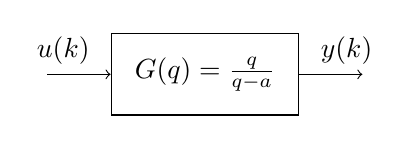
\begin{tikzpicture}[node distance=20mm, anchor=north]
\node[coordinate] (input) {};
\node[rectangle, draw, right of=input, inner sep=3mm] (lti) {$G(q)=\frac{q}{q-a}$};
\node[coordinate, right of=lti] (output) {};
\draw[->] (input) -- node[near start, above] {$u(k)$}  (lti);
\draw[->] (lti) -- node[near end, above] {$y(k)$} (output);
\end{tikzpicture}
\end{center}

The system with pulse-transfer operator \(G(q)=\frac{q}{q-a}\) corresponds to the difference equation
\[ y(k) = G(q)u(k) \Leftrightarrow y(k) = \frac{q}{q-a} u(k) \]
\[ y(k+1) = ay(k) + u(k+1). \quad \text{If $a=1$, the system is a discrete-time integrator}\]
\end{frame}


\begin{frame}[label={sec:org24eddd6}]{Impulse-response of a first order system}
\[ y(k+1) = ay(k) + u(k+1), \quad y(k)=0, \; k<0 \]
\[ u(k) = \delta(k) = \begin{cases} 1, & k=1\\ 0, & \text{otherwise}\end{cases} \]

\begin{block}{Solution}
\begin{align*}
y(0) &= ay(-1) + u(0) = 1\\
y(1) &= ay(0) + u(1) = a + 0 = a\\
y(2) &= ay(1) + u(2) = a*a + 0 = a^2\\
     &\vdots\\
y(n) &= a^n
\end{align*}
\end{block}
\end{frame}

\begin{frame}[label={sec:org5f1dd72}]{Impulse response of a first order system}
\[ y(k+1) = ay(k) + u(k+1) \]

\alert{Activity} Pair the impulse response to each of the values of \(a\)
\[ \text{I)}\; a=1 \qquad \text{II)}\; a=2 \qquad \text{III)}\; a = 0.5 \qquad \text{IV)}\; a=-0.9 \]

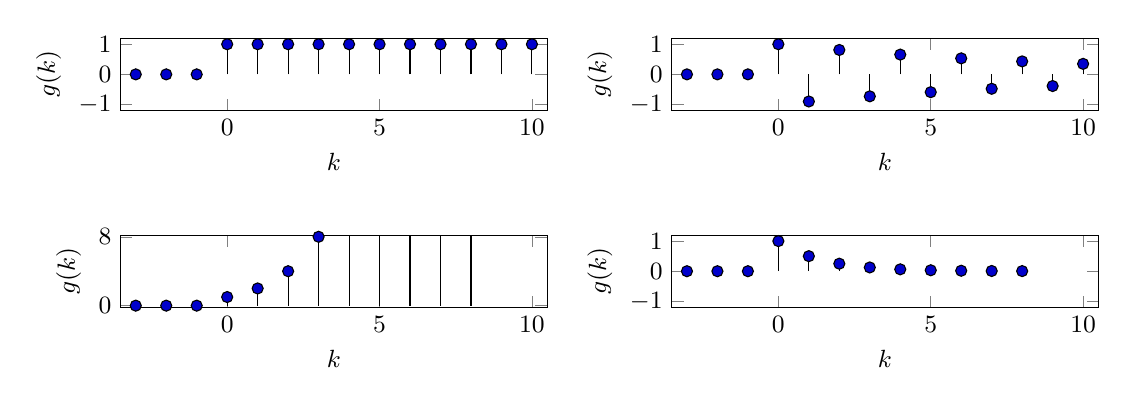
\begin{tikzpicture}
\small
\begin{axis}[
width=7cm,
height=2.5cm,
xlabel={$k$},
ylabel={$g(k)$},
xmin=-3.5,
xmax=10.5,
ytick = {-1,0,1},
ymin = -1.2, ymax=1.2,
]
\addplot+[black, ycomb, domain=-3:10, samples=14,variable=k] { (k>=0)*pow(1,k)};
\end{axis}

\begin{axis}[
xshift=7cm,
width=7cm,
height=2.5cm,
xlabel={$k$},
ylabel={$g(k)$},
xmin=-3.5,
xmax=10.5,
ytick = {0},
ytick = {-1,0,1},
ymin = -1.2, ymax=1.2,
]
\addplot+[black, ycomb, domain=-3:10, samples=14,variable=k] { (k>=0)*pow(-0.9,k)};
\end{axis}

\begin{axis}[
xshift=0cm,
yshift=-2.5cm,
width=7cm,
height=2.5cm,
xlabel={$k$},
ylabel={$g(k)$},
xmin=-3.5,
xmax=10.5,
ytick = {0},
ytick = {-1,0,8},
ymin = -0.2, ymax=8.2,
]
\addplot+[black, ycomb, domain=-5:8, samples=14,variable=k] {  (k>=0)*pow(2,k) };
\end{axis}

\begin{axis}[
xshift=7cm,
yshift=-2.5cm,
width=7cm,
height=2.5cm,
xlabel={$k$},
ylabel={$g(k)$},
xmin=-3.5,
xmax=10.5,
ytick = {0},
ytick = {-1,0,1},
ymin = -1.2, ymax=1.2,
]
\addplot+[black, ycomb, domain=-5:8, samples=14,variable=k] {  (k>=0)*pow(0.5,k)};
\end{axis}


\end{tikzpicture}
\end{frame}
\end{document}